\documentclass{beamer}
\usepackage{graphicx}
\mode<presentation> { \usetheme{Madrid} }

\title{Kotlin\texorpdfstring{$\nabla$}{}}
\subtitle{Differentiable functional programming with algebraic data types}
\author{Breandan Considine}
\institute[UdeM]{
Universit\'e de Montr\'eal \\
\medskip
\textit{breandan.considine@umontreal.ca}
}
\date{\today}

\begin{document}
    \begin{frame}
        \titlepage
    \end{frame}

    \begin{frame}
        \frametitle{Overview}
        \tableofcontents
    \end{frame}

    \section{Introduction and motivation}\label{sec:first-section}

    \begin{frame}
        \frametitle{Kotlin}
        \begin{itemize}
            \item Goal: To implement automatic differentiation in Kotlin
            \item Kotlin is a JVM language with emphasis on type and null safety
            \item Offers features for building domain specific languages (DSLs)
            \item Supports first-class functions, higher order functions and FP
            \item Has support for extension functions and algebraic data types
            \item Operator overloading and other syntactic sugar (to be shown)
        \end{itemize}
    \end{frame}


    \begin{frame}
        \frametitle{$y = \frac{\sin{\sin{\sin{x}}}}{x} + x \sin{x} + \cos{x} + x$, $\frac{dy}{dx}$, $\frac{d^{2}y}{dx^2}$, $\frac{d^{3}y}{dx^3}$, $\frac{d^{4}y}{dx^4}$, $\frac{d^{5}y}{dx^5}$}
        \begin{center}
            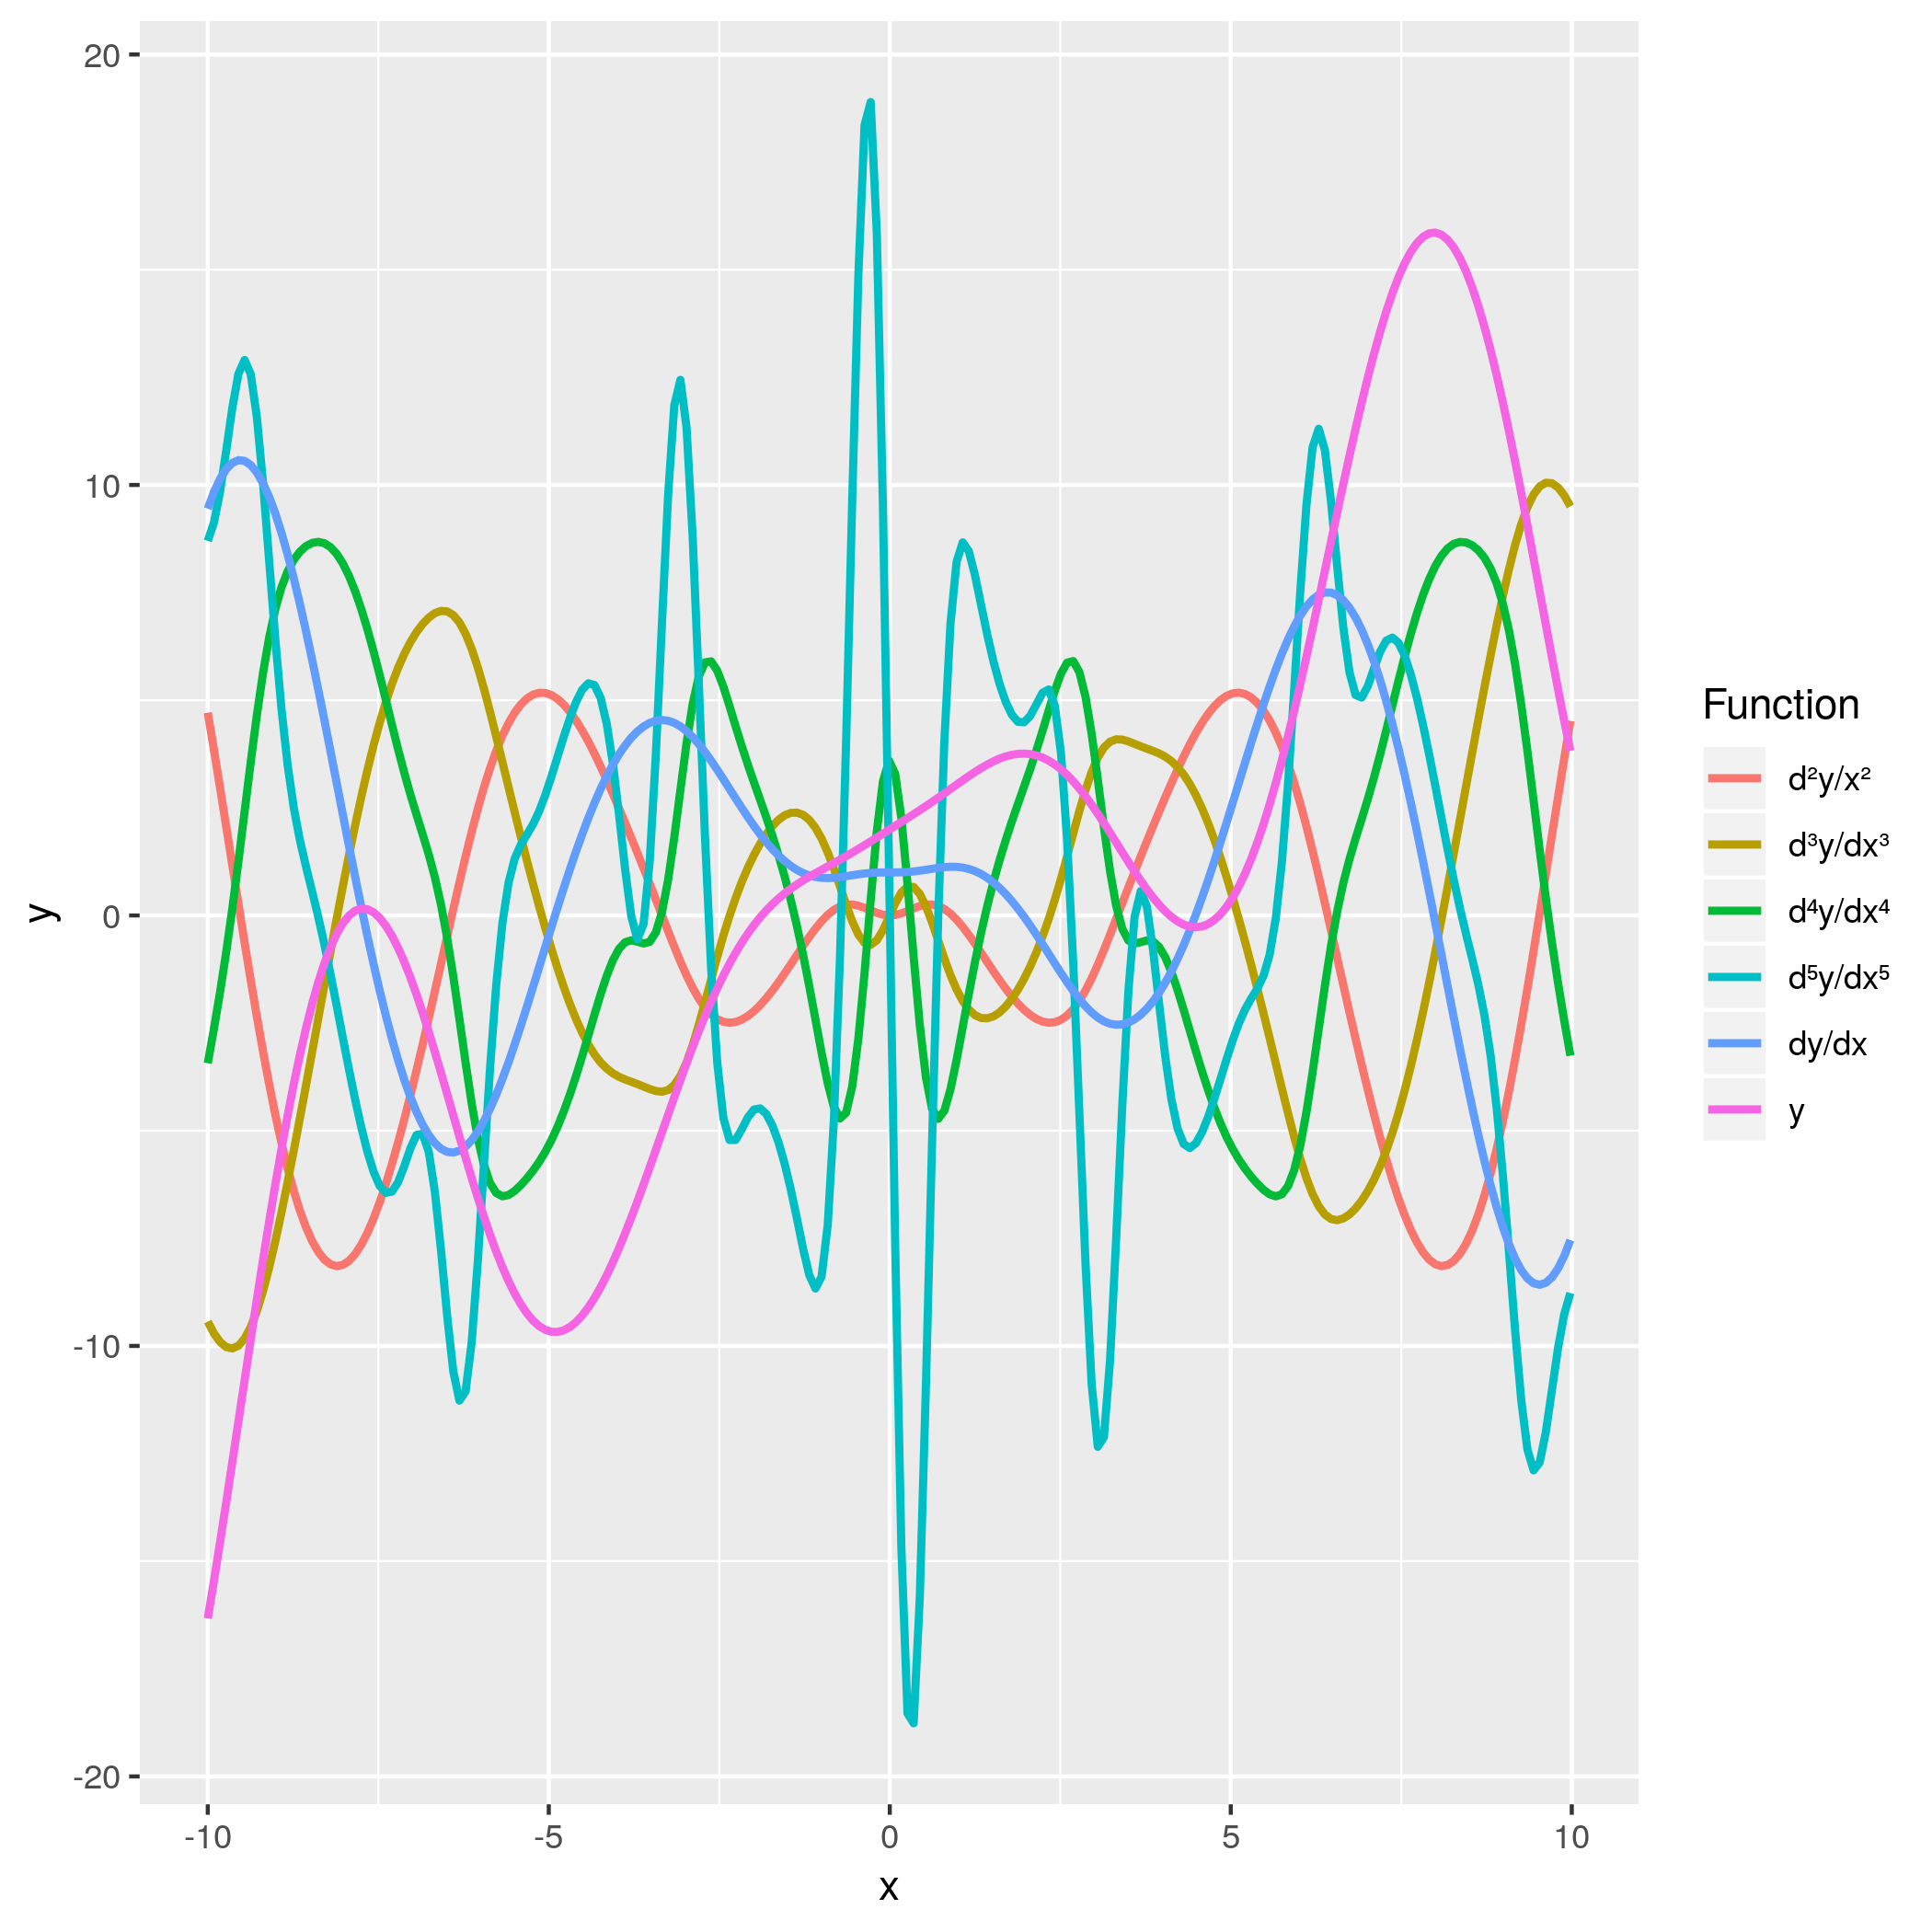
\includegraphics[scale=0.4]{plot.png}
        \end{center}
    \end{frame}

    \begin{frame}
        \frametitle{Kotlin\texorpdfstring{$\nabla$}{}}
        \begin{itemize}
            \item
            \item Type system from algebraic first principles (group, ring, field)
            \item Automatic differentiation using a natural (infix) notation
            \item Supports partials and higher order derivatives, gradients
            \item Property-based testing using finite differences (Hypothesis, QuickCheck)
        \end{itemize}
    \end{frame}

    \section{A Short History of Computing Derivatives}\label{sec:second-section}

    %------------------------------------------------------------------------------------------------

    \begin{frame}
        \frametitle{Numerical differentiation}
        \begin{itemize}
            \item Many mathematical formula have discrete, numerical representations
            \item But numerical values can be an \textit{inexact} representation of math
            \item Long calculations on primitives are susceptible to rounding errors
            \item Bag of tricks for discrete approximation and numerical stability:
            \begin{itemize}
                \item Fourier, Chebyshev, Lagrange
                \item Arbitrary precision arithmetic
                \item Kahan summation algorithm
                \item log-sum-exp trick
            \end{itemize}
        \end{itemize}
    \end{frame}

    %------------------------------------------------------------------------------------------------

    \begin{frame}
        \frametitle{Symbolic differentiation}
        \begin{itemize}
            \item What about evaluating functions symbolically?
            \item Computer algebra systems for manipulate symbolic formulas
        \end{itemize}
    \end{frame}

    %------------------------------------------------------------------------------------------------

    \begin{frame}
        \frametitle{Automatic differentiation}
        \begin{itemize}
            \item Derivatives can be calculated automatically? (Wengert, 1964)
            \item Code as an \textit{exact} symbolic representation of functions
            \item To reason about code we need the ability to treat \textit{code as data}:
            \begin{itemize}
                \item Reflection and metaprogramming
                \item Domain specific languages
                \item First-class functions
            \end{itemize}
        \end{itemize}
    \end{frame}

    %------------------------------------------------------------------------------------------------

    \begin{frame}
        \frametitle{Differentiable [functional] programming}
        \begin{itemize}
            \item What is a program, but a series of arithmetic operations?
            \item What are arithmetic operations but syntactic sugar for functions?
            \item Functions can be composed of other functions or chained in sequence
            \item High school calculus gives us rules for differentiating function chains
            \item Pearlmutter \& Siskind teach us AD is possible just using FP (2016)
            \item Wang, Rompf, et al. show us this is possible \textit{without a tape}! (2018)
        \end{itemize}
    \end{frame}

    %------------------------------------------------------------------------------------------------

    \begin{frame}
        \frametitle{Differentiable programming with algebraic types}
        \begin{itemize}
            \item Combine the tools from mathematics and CS
            \item Type safety
            \item Static analysis
            \item Allows us to preserve symmetries that are not obvious
            \item There is an abstract algebra for tensor manipulations
            \item Can be encoded using OOP and parametric polymorphism
            \item \href{https://arxiv.org/pdf/1610.07690.pdf}{Operational Calculus for Differentiable Programming}
        \end{itemize}
    \end{frame}

    %------------------------------------------------------------------------------------------------


    \begin{frame}
        \frametitle{Not reinventing the wheel}
        \begin{itemize}
            \item Haskell already does this: Group
            \item Parsing expressions in a FP
        \end{itemize}
    \end{frame}

    %------------------------------------------------------------------------------------------------

    \section{Architectural Overview}\label{sec:third-section}

    \begin{frame}
        \frametitle{Architecture}
    \end{frame}

    \section{Usage}\label{sec:fourth-section}

    \begin{frame}
        \frametitle{Usage}
    \end{frame}

    \section{Future Plans}\label{sec:fifth-section}

    \begin{frame}
        \frametitle{Roadmap}
        \item TODO
    \end{frame}

    \begin{frame}
        \frametitle{Further directions to explore}
        \begin{itemize}
            \item Closer integration with Kotlin/Java standard library
            \item \href{https://discuss.kotlinlang.org/t/primitive-type-specialization/11022/4}{Primitive type specialization}
            \item Use \href{https://arrow-kt.io/}{Arrow} for truly native functional programming
            \item Dependent types via code generation to type check tensor shapes
            \item Encode additional structure like arity into the type system
            \item Performance benchmarks and zero-cost un/boxing abstractions
            \item Lazy evaluation and configurable forward/backward AD modes
            \item Automatic expression refactoring for numerical stability
        \end{itemize}
    \end{frame}

\end{document}

% %----------------------------------------------------------------------------------------
% %	PRESENTATION SLIDES
% %----------------------------------------------------------------------------------------

% %------------------------------------------------
% \section{First Section}

% %------------------------------------------------

% \subsection{Subsection Example} % A subsection can be created just before a set of slides with a common theme to further break down your presentation into chunks

% \begin{frame}
% \frametitle{Paragraphs of Text}
% Sed iaculis dapibus gravida. Morbi sed tortor erat, nec interdum arcu. Sed id lorem lectus. Quisque viverra augue id sem ornare non aliquam nibh tristique. Aenean in ligula nisl. Nulla sed tellus ipsum. Donec vestibulum ligula non lorem vulputate fermentum accumsan neque mollis.\\~\\

% Sed diam enim, sagittis nec condimentum sit amet, ullamcorper sit amet libero. Aliquam vel dui orci, a porta odio. Nullam id suscipit ipsum. Aenean lobortis commodo sem, ut commodo leo gravida vitae. Pellentesque vehicula ante iaculis arcu pretium rutrum eget sit amet purus. Integer ornare nulla quis neque ultrices lobortis. Vestibulum ultrices tincidunt libero, quis commodo erat ullamcorper id.
% \end{frame}

% %------------------------------------------------

% \begin{frame}
% \frametitle{Bullet Points}
% \begin{itemize}
% \item Lorem ipsum dolor sit amet, consectetur adipiscing elit
% \item Aliquam blandit faucibus nisi, sit amet dapibus enim tempus eu
% \item Nulla commodo, erat quis gravida posuere, elit lacus lobortis est, quis porttitor odio mauris at libero
% \item Nam cursus est eget velit posuere pellentesque
% \item Vestibulum faucibus velit a augue condimentum quis convallis nulla gravida
% \end{itemize}
% \end{frame}

% %------------------------------------------------

% \begin{frame}
% \frametitle{Blocks of Highlighted Text}
% \begin{block}{Block 1}
% Lorem ipsum dolor sit amet, consectetur adipiscing elit. Integer lectus nisl, ultricies in feugiat rutrum, porttitor sit amet augue. Aliquam ut tortor mauris. Sed volutpat ante purus, quis accumsan dolor.
% \end{block}

% \begin{block}{Block 2}
% Pellentesque sed tellus purus. Class aptent taciti sociosqu ad litora torquent per conubia nostra, per inceptos himenaeos. Vestibulum quis magna at risus dictum tempor eu vitae velit.
% \end{block}

% \begin{block}{Block 3}
% Suspendisse tincidunt sagittis gravida. Curabitur condimentum, enim sed venenatis rutrum, ipsum neque consectetur orci, sed blandit justo nisi ac lacus.
% \end{block}
% \end{frame}

% %------------------------------------------------

% \begin{frame}
% \frametitle{Multiple Columns}
% \begin{columns}[c] % The "c" option specifies centered vertical alignment while the "t" option is used for top vertical alignment

% \column{.45\textwidth} % Left column and width
% \textbf{Heading}
% \begin{enumerate}
% \item Statement
% \item Explanation
% \item Example
% \end{enumerate}

% \column{.5\textwidth} % Right column and width
% Lorem ipsum dolor sit amet, consectetur adipiscing elit. Integer lectus nisl, ultricies in feugiat rutrum, porttitor sit amet augue. Aliquam ut tortor mauris. Sed volutpat ante purus, quis accumsan dolor.

% \end{columns}
% \end{frame}

% %------------------------------------------------
% \section{Second Section}
% %------------------------------------------------

% \begin{frame}
% \frametitle{Table}
% \begin{table}
% \begin{tabular}{l l l}
% \toprule
% \textbf{Treatments} & \textbf{Response 1} & \textbf{Response 2}\\
% \midrule
% Treatment 1 & 0.0003262 & 0.562 \\
% Treatment 2 & 0.0015681 & 0.910 \\
% Treatment 3 & 0.0009271 & 0.296 \\
% \bottomrule
% \end{tabular}
% \caption{Table caption}
% \end{table}
% \end{frame}

% %------------------------------------------------

% \begin{frame}
% \frametitle{Theorem}
% \begin{theorem}[Mass--energy equivalence]
% $E = mc^2$
% \end{theorem}
% \end{frame}

% %------------------------------------------------

% \begin{frame}[fragile] % Need to use the fragile option when verbatim is used in the slide
% \frametitle{Verbatim}
% \begin{example}[Theorem Slide Code]
% \begin{verbatim}
% \begin{frame}
% \frametitle{Theorem}
% \begin{theorem}[Mass--energy equivalence]
% $E = mc^2$
% \end{theorem}
% \end{frame}\end{verbatim}
% \end{example}
% \end{frame}

% %------------------------------------------------

% \begin{frame}
% \frametitle{Figure}
% Uncomment the code on this slide to include your own image from the same directory as the template .TeX file.
% %\begin{figure}
% %\includegraphics[width=0.8\linewidth]{test}
% %\end{figure}
% \end{frame}

% %------------------------------------------------

% \begin{frame}[fragile] % Need to use the fragile option when verbatim is used in the slide
% \frametitle{Citation}
% An example of the \verb|\cite| command to cite within the presentation:\\~

% This statement requires citation \cite{p1}.
% \end{frame}

% %------------------------------------------------

% \begin{frame}
% \frametitle{References}
% \footnotesize{
% \begin{thebibliography}{99} % Beamer does not support BibTeX so references must be inserted manually as below
% \bibitem[Smith, 2012]{p1} John Smith (2012)
% \newblock Title of the publication
% \newblock \emph{Journal Name} 12(3), 45 -- 678.
% \end{thebibliography}
% }
% \end{frame}

% %------------------------------------------------

% \begin{frame}
% \Huge{\centerline{The End}}
% \end{frame}

% %------------------------------------------------